% Created 2021-10-06 mar 13:05
% Intended LaTeX compiler: pdflatex
%%% Local Variables:
%%% LaTeX-command: "pdflatex --shell-escape"
%%% End:
\documentclass[11pt]{article}
\usepackage[utf8]{inputenc}
\usepackage[T1]{fontenc}
\usepackage{graphicx}
\usepackage{grffile}
\usepackage{longtable}
\usepackage{wrapfig}
\usepackage{rotating}
\usepackage[normalem]{ulem}
\usepackage{amsmath}
\usepackage{textcomp}
\usepackage{amssymb}
\usepackage{listings}
\usepackage{capt-of}
\usepackage{hyperref}
\hypersetup{colorlinks=true, linkcolor=black}
\setlength{\parindent}{0in}
\usepackage[margin=1.1in]{geometry}
\usepackage[spanish]{babel}
\usepackage{mathtools}
\usepackage{palatino}
\usepackage{fancyhdr}
\usepackage{sectsty}
\usepackage{engord}
\usepackage{cite}
\usepackage{graphicx}
\usepackage{setspace}
\usepackage[compact]{titlesec}
\usepackage[center]{caption}
\usepackage{placeins}
\usepackage{tikz}
\usetikzlibrary{positioning}
\usetikzlibrary{bayesnet}
\usetikzlibrary{shapes.geometric}
\usetikzlibrary{decorations.text}
\usepackage{color}
\usepackage{amsmath}
\usepackage{minted}
\usepackage{pdfpages}



\def\inline{\lstinline[basicstyle=\ttfamily,keywordstyle={}]}
\newtheorem{theorem}{Theorem}
\titlespacing*{\subsection}{0pt}{5.5ex}{3.3ex}
\titlespacing*{\section}{0pt}{5.5ex}{1ex}
\author{José Antonio Álvarez Ocete\\ Francisco Javier Sáez Maldonado}
\date{\today}
\title{Introducción a Hadoop y Spark\\ Procesamiento de Datos a Gran Escala}

\newcommand{\I}{\mathbb{I}}
\newcommand{\la}{\langle}
\newcommand{\ra}{\rangle}

\begin{document}

\maketitle

\tableofcontents

Dividiremos esta práctica en 2 partes fundamentales. 

\begin{enumerate}
	
	\item En la primera, se concentrará en realizar diversas pruebas con los elementos más básicos de la programación en CUDA.
	\item En la segunda, TODO!!!!!!!!!!!
\end{enumerate}

\section{Parte 1: Programación GPGPU}

\subsection{Recursos de la GPU}

Para programar en GPU, el primer paso que debemos dar es conocer las características (y por tanto, los recursos) que el dispositivo del que disponemos nos ofrece. En este caso práctico, vamos a realizar las pruebas utilizando \href{https://colab.research.google.com/}{Google Colaboratory}. Google pone a disposición del usuario tanto GPUs como TPUs que son más que suficientes para realizar algunas pruebas. 

Lo primero que haremos es estudiar qué recursos tiene el equipo que nos ofrece Google. la GPU que nos ofrecen desde Google. Podemos ejecutar el comando \inline{!lscpu} para obtener información sobre el modelo de CPU que tenemos. El resultado nos muestra que tenemos un procesador \emph{Intel(R) Xeon(R) CPU @ 2.30GHz} de 64 bits. Además, si ejecutamos \inline{!free -kh} vemos que tenemos los siguientes recursos disponibles:
\begin{minted}[fontsize=\footnotesize]{bash}
	total        used        free      shared  buff/cache   available
Mem:            12G        571M        9.9G        1.2M        2.2G         11G
Swap:            0B          0B          0B
\end{minted}

Como vemos, tenemos 12Gb de memoria prácticamente disponibles. Ahora, queremos comprobar también los recursos GPU que tenemos disponibles, sabiendo que hemos activado el entorno de Colaboratory para que tenga GPU. Verificamos las tarjetas gráficas que tenemos utilizando la orden \inline{nvidia-smi}. Obtenemos el resultado siguiente:\\

\begin{minipage}{0.7\textwidth}

\begin{minted}[fontsize=\footnotesize]{bash}
	Fri Oct 29 14:57:32 2021       
+-----------------------------------------------------------------------------+
| NVIDIA-SMI 495.29.05    Driver Version: 460.32.03    CUDA Version: 11.2     |
|-------------------------------+----------------------+----------------------+
| GPU  Name        Persistence-M| Bus-Id        Disp.A | Volatile Uncorr. ECC |
| Fan  Temp  Perf  Pwr:Usage/Cap|         Memory-Usage | GPU-Util  Compute M. |
|                               |                      |               MIG M. |
|===============================+======================+======================|
|   0  Tesla K80           Off  | 00000000:00:04.0 Off |                    0 |
| N/A   48C    P8    30W / 149W |      0MiB / 11441MiB |      0%      Default |
|                               |                      |                  N/A |
+-------------------------------+----------------------+----------------------+
                                                                               
+-----------------------------------------------------------------------------+
| Processes:                                                                  |
|  GPU   GI   CI        PID   Type   Process name                  GPU Memory |
|        ID   ID                                                   Usage      |
|=============================================================================|
|  No running processes found                                                 |
+-----------------------------------------------------------------------------+
\end{minted}
\end{minipage}\\
Como vemos, en \textbf{esta conexión al servidor} se nos ha proporcionado una \emph{Nvidia Tesla K80}. Hacemos hincapié en que es en esta conexión porque en Google Colaboratory se asigna una GPU que esté disponible en ese momento, por lo que en otra ejecución podríamos obtener otra de capacidades de computación similares.

Además de eso, se nos indica que tenemos como driver instalado la versión \inline{11.2} de CUDA. Sin embargo, hemos comprobado que la versión de ejecución de CUDA no es la misma de dos maneras distintas. Primeramente, si hacemos \lstinline{!nvcc --version} ya se nos indica por primera vez lo siguiente:
\begin{minted}[]{bash}
Cuda compilation tools, release 11.1, V11.1.105
Build cuda_11.1.TC455_06.29190527_0
\end{minted}

Además de eso, podemos compilar el ejemplo que tenemos en \\ \lstinline{/usr/local/cuda/samples/1_Utilities/deviceQuery/} usando el \inline{makefile} proporcionado y, al ejecutar el ejemplo, obtenemos la siguiente salida (mostramos un resumen de la misma debido a su extensión):
\begin{minted}[]{bash}
Device 0: "Tesla K80"
  CUDA Driver Version / Runtime Version          11.2 / 11.1
  ... 
  Total amount of constant memory:               65536 bytes
  Total amount of shared memory per block:       49152 bytes
  Total shared memory per multiprocessor:        114688 bytes
  Total number of registers available per block: 65536
  Warp size:                                     32
  Maximum number of threads per multiprocessor:  2048
  Maximum number of threads per block:           1024
  Max dimension size of a thread block (x,y,z): (1024, 1024, 64)
  Max dimension size of a grid size    (x,y,z): (2147483647, 65535, 65535)
  ... 
\end{minted}


Como datos a destacar, vemos que tenemos 65536 registros disponibles por bloque, con un tamaño de Warp de $32$ y con un máximo número de hilos por bloque de $1024$. Estos datos tendrán implicaciones a la hora de hacer ejecuciones.  Además, viendo la dimensión máxima de un grid en la tripla que se nos ofrece, obtenemos que el número máximo de bloque es $65535$.


\subsection{Suma de 2 vectores}

Construiremos en varias etapas un programa en CUDA que realiza la suma de dos vectores.

\subsubsection{Suma de dos enteros}

Comenzamos con un ejemplo sencillo de cálculo de una suma de enteros usando CUDA. El código está proporcionado en el cuaderno de enunciado de la práctica. Explicamos brevemente el código para entender mejor las preguntas:

\begin{minted}[]{CUDA}
__global__ void add(int *a, int *b, int *c) {
	*c = *a + *b;
}
\end{minted}
Este bloque implementa la función suma de dos enteros que se pasan como un puntero. Se almacena el valor de la suma en un tercer puntero que se pasa a la función.

\begin{minted}[]{CUDA}
// host copies of variables a, b & c
int a, b, c;

// device copies of variables a, b & c  
int *d_a, *d_b, *d_c;

int size = sizeof(int);
// Allocate space for device copies of a, b, c
cudaMalloc((void **)&d_a, size);
cudaMalloc((void **)&d_b, size);
cudaMalloc((void **)&d_c, size);
// Setup input values  
c = 0;
a = 3;
b = 5;
\end{minted}
En este bloque se hace la declaración de variables. Se hacen tres variables, luego se declaran punteros a tres variables y se declara un entero \inline{size} que tiene como valor el tamaño de un entero. A continuación, se declaran en CUDA punteros (usando los tres punteros declarados anteriormente) de tamaño \inline{size}. Por último, se le da valor a los enteros para poder sumarlos.

\begin{minted}[]{CUDA}
// Copy inputs to device
cudaMemcpy(d_a, &a, size, cudaMemcpyHostToDevice);
cudaMemcpy(d_b, &b, size, cudaMemcpyHostToDevice);

// Launch add() kernel on GPU
add<<<1,1>>>(d_a, d_b, d_c);  
\end{minted}
En este fragmento, primero se copia a la memoria de la GPU las referencias a los enteros que hemos inicializado anteriormente, es decir, ahora en la memoria de CUDA los punteros inicializados en cuda apuntan a la misma posición de memoria que tiene en el disco los valores que se quieren sumar. Se usa el valor \inline{cudaMemcpyHostToDevice} del enumerado \inline{cudaMemcpyKind} que indica que el valor irá desde el Host (el equipo) al Device (la GPU). A continuación, se realiza la operación suma \inline{add<<<1,1>>>} indicándole que se haga con 1 bloque y 1 hebra. 

\begin{minted}[]{CUDA}
// Copy result back to host
cudaError err = cudaMemcpy(&c, d_c, size, cudaMemcpyDeviceToHost);
if(err!=cudaSuccess) 
	printf("CUDA error copying to Host: %s\n", cudaGetErrorString(err));

printf("result is %d\n",c);
// Cleanup
cudaFree(d_a);
cudaFree(d_b);
cudaFree(d_c);
\end{minted}

En este último código, se hace apuntar el puntero que tiene el resultado en la GPU al puntero que tiene la memoria del dispositivo, guardando si ha habido algún error. Ahora, se usa otro valor del enumerado: \inline{cudaMemcpyDeviceToHost}, que indica que el valor vaya desde la GPU al equipo. Finalmente, se liberan de la GPU los espacios reservados para los punteros. El resultado de la ejecución es el esperado.

\begin{minted}[]{bash}
!./suma1d

result is 8
\end{minted}

Si comprobamos el perfil de ejecución, vemos el siguiente resultado:

\begin{minted}[fontsize=\footnotesize]{bash}
	==229== NVPROF is profiling process 229, command: ./suma1d
==229== Warning: Auto boost enabled on device 0. Profiling results may be inconsistent.
result is 8
==229== Profiling application: ./suma1d
==229== Profiling result:
            Type  Time(%)      Time     Calls       Avg       Min       Max  Name
 GPU activities:   37.50%  3.7440us         2  1.8720us  1.5040us  2.2400us  [CUDA memcpy HtoD]
                   36.54%  3.6480us         1  3.6480us  3.6480us  3.6480us  add(int*, int*, int*)
                   25.96%  2.5920us         1  2.5920us  2.5920us  2.5920us  [CUDA memcpy DtoH]
      API calls:   99.56%  270.53ms         3  90.177ms  2.6620us  270.52ms  cudaMalloc
                    0.21%  565.39us         1  565.39us  565.39us  565.39us  cuDeviceTotalMem
                    0.12%  321.01us       101  3.1780us     210ns  140.66us  cuDeviceGetAttribute
                    0.06%  171.37us         3  57.124us  5.6250us  152.77us  cudaFree
                    0.02%  60.590us         3  20.196us  11.684us  25.788us  cudaMemcpy
                    0.01%  32.193us         1  32.193us  32.193us  32.193us  cuDeviceGetName
                    0.01%  24.277us         1  24.277us  24.277us  24.277us  cudaLaunchKernel
                    0.00%  5.0420us         1  5.0420us  5.0420us  5.0420us  cuDeviceGetPCIBusId
                    0.00%  1.9970us         3     665ns     186ns  1.0810us  cuDeviceGetCount
                    0.00%  1.5280us         2     764ns     401ns  1.1270us  cuDeviceGet
                    0.00%     420ns         1     420ns     420ns     420ns  cuDeviceGetUuid
\end{minted}

Como vemos, tenemos una única llamada a la función \inline{add}, $3$ llamadas a la función \inline{cudaMalloc} y otras tres para copiar las referencias usando \inline{cudaMemcpy}. Podemos observar en esta primera ejecución cómo se hacen $101$ llamadas a \inline{cuDeviceGetAttribute}, que nos devuelve un valor que se almacena en la memoria de la GPU.

\subsubsection{Paralelizando}
\subsubsection*{Sumando vectores}

El objetivo ahora será modificar el código actual para que la suma de vectores se realice según los bloques y las hebras que se le indiquen. En particular, querremos modificar el número de hebras para que se puedan paralelizar las operaciones. Comenzamos cambiando el número de hebras a $512$. Podemos apreciar en el código de la suma un cambio:
\begin{minted}{CUDA}
__global__ void add(int *a, int *b, int *c) {
    //*c = *a + *b;
    c[blockIdx.x] = a[blockIdx.x] + b[blockIdx.x];
}
\end{minted}

Ahora, accedemos al valor \inline{blockIdx.x} de cada uno de los punteros para realizar la suma. Esto es importante pues ahora querremos que cada operación la realice un bloque. Generalizamos el programa anterior para que sume vectores del mismo tamaño, elemento a elemento.

\begin{minted}[]{CUDA}
int *a, *b, *c;        // host copies of variables a, b & c
int *d_a, *d_b, *d_c;  // device copies of variables a, b & c
int size = N * sizeof(int);
// Allocate space for host copies of a, b, c   Setup inputvalues  
a =  (int *) malloc(size); 
b =  (int *) malloc(size); 
c =  (int *) malloc(size); 
//   Setup input values  
for( int i = 0; i < N; i++ ){
	a[i] = i;
  	b[i] = N-i;
	c[i] = 0;
}	
\end{minted}

Como vemos, la inicialización de los valores es diferente. Ahora necesitamos dejar espacio en el disco que tenga tamaño: el tamaño del vector por lo que ocupa un entero. Entonces, la inicialización se hace en un bucle \inline{for}.
\begin{minted}[]{CUDA}
cudaMalloc((void **)&d_a, size);
cudaMalloc((void **)&d_b, size);
cudaMalloc((void **)&d_c, size);
// Copy inputs to device
cudaMemcpy(d_a, a, size, cudaMemcpyHostToDevice);
cudaMemcpy(d_b, b, size, cudaMemcpyHostToDevice);
\end{minted}

Se reservan en memoria espacio para los vectores y se copian a la GPU usando la misma función, solo que asignando más espacio mediante el parámetro \inline{size}.

\begin{minted}[]{CUDA}
// Launch add() kernel on GPU  Se lanzan N bloques de 1 Thread.
add<<<N,1>>>(d_a, d_b, d_c);
\end{minted}
Se realiza la operación suma entre los dos vectores. Llamándola de la forma \inline{add<<<N,M>>>} estamos indicando que queremos realizar la operación usando $N$ bloques y $M$ hebras. En este caso concreto, estaríamos diciendo que se haga la operación con $N = 512$ (definido como variable del programa) bloques y $1$ hebra.

El resultado final del programa es el siguiente:
\begin{minted}[]{bash}
valor a[0] es 0
valor b[0] es 512
resultado c[0] es 512
valor a[2] es 2
valor b[2] es 510
resultado c[2] es 512	
\end{minted}

Como podemos ver, todo parece estar ocurriendo en orden. Añadimos un bucle for que comprueba si todos los valores del vector \inline{c} valen lo mismo, y lo imprime por pantalla:
\begin{minted}[]{CUDA}
bool res = 1;
for(int i  = 0; i < N; i++)
  if(c[i] != N)
	res = 0;

printf("Todos los valores de c valen lo mismo (1 true, 0 false):%d\n",res);
... 
Todos los valores de c valen lo mismo (1 true, 0 false): 1
\end{minted}
Como vemos, el resultado es correcto. Vemos el perfil de ejecución en este caso:
\begin{minted}[fontsize=\footnotesize]{bash}
==1891== NVPROF is profiling process 1891, command: ./suma2dvector
==1891== Warning: Auto boost enabled on device 0. Profiling results may be inconsistent.
 valor a[0] es 0
 valor b[0] es 512
resultado c[0] es 512
 valor a[2] es 2
 valor b[2] es 510
resultado c[2] es 512
Todos los valores de c valen lo mismo (1 true, 0 false): 1
==1891== Profiling application: ./suma2dvector
==1891== Profiling result:
	Type  Time(%)      Time     Calls       Avg       Min       Max  Name
GPU:    40.98%  5.0880us         1  5.0880us  5.0880us  5.0880us  add(int*, int*, int*)
        37.63%  4.6720us         2  2.3360us  2.0160us  2.6560us  [CUDA memcpy HtoD]
        21.39%  2.6560us         1  2.6560us  2.6560us  2.6560us  [CUDA memcpy DtoH]
API calls:  99.49%  190.44ms         3  63.479ms  2.2440us  190.43ms  cudaMalloc
		0.28%  529.05us         1  529.05us  529.05us  529.05us  cuDeviceTotalMem
		0.10%  199.48us       101  1.9750us     145ns  87.079us  cuDeviceGetAttribute
		0.07%  134.29us         3  44.764us  3.2210us  115.10us  cudaFree
		0.03%  56.462us         3  18.820us  11.545us  25.237us  cudaMemcpy
		0.01%  26.486us         1  26.486us  26.486us  26.486us  cuDeviceGetName
		0.01%  25.925us         1  25.925us  25.925us  25.925us  cudaLaunchKernel
		0.00%  5.9010us         1  5.9010us  5.9010us  5.9010us  cuDeviceGetPCIBusId
		0.00%  1.7020us         3     567ns     162ns     876ns  cuDeviceGetCount
		0.00%  1.2500us         2     625ns     233ns  1.0170us  cuDeviceGet
		0.00%     385ns         1     385ns     385ns     385ns  cuDeviceGetUuid
\end{minted}

Como vemos, de nuevo tenemos una única llamada a la función \inline{add}. No se observa una diferencia apreciable entre el tiempo de ejecución de esta llamada en este caso y en el anterior. Tampoco en el resto de operaciones que se hacen en la GPU.

\subsubsection*{1 Bloque - N Threads}

El objetivo será usar la modificación del programa que utiliza en un solo bloque $N$ hebras para paralelizar la ejecución. Habíamos definido antes $N=512$ para usar ese número de bloques. Ahora, se redefine como $N=1024$ para usar este número de hebras (que vimos en la descripción de la GPU que es el número máximo).

Al igual que en el caso anterior, la función suma cambia:

\begin{minted}[]{CUDA}
__global__ void add(int *a, int *b, int *c) {
	c[threadIdx.x] = a[threadIdx.x] + b[threadIdx.x]; 
}
\end{minted}

Como vemos, ahora se accede al índice de la hebra usando \inline{threadIdx.x}. Otro cambio que se debe hacer claramente es que la función add se llame de la forma:
\begin{minted}[]{CUDA}
// Launch add() kernel on GPU  Se lanzan 1 bloques de N Threads.
add<<<1,N>>>(d_a, d_b, d_c);
\end{minted}
Volvemos a mostrar el resultado de la ejecución de este nuevo programa.
\begin{minted}[]{bash}
valor a[10] es 10
valor b[10] es 1014
resultado c[10] es 1024
valor a[0] es 0
valor b[0] es 1024
resultado c[0] es 1024
Todos los valores de c valen lo mismo (1 true, 0 false): 1	
\end{minted}

Se aprecia que todos los resultados son correctos. Se pide de nuevo que se compare el perfil de ejecución con los anteriores, pero no se aprecia ninguna diferencia significativa en los resultados.

\subsubsection{Preguntas}

\begin{enumerate}

\item Pruebe a lanzar diferente número de Threads ( con un solo 1 bloque)
  ¿Cual son los valores máximos y mínimos de número de theads por bloque en esta GPU?\\

  Estos valores mínimos ya se podían observar cuando ejecutábamos el programa \inline{deviceQuery}. En él, aparecía que el número máximo de threads por bloque era $1024$. Ya hemos mostrado que, en el caso de ejecutarlo con este número los resultados son correctos.

  \begin{minted}[]{bash}
	add<<<1,1025>>>(d_a, d_b, d_c);
	... 
	valor a[10] es 10
 	valor b[10] es 1014
	resultado c[10] es 0
 	valor a[0] es 0
 	valor b[0] es 1024
	resultado c[0] es 0
	Todos los valores de c valen lo mismo (1 true, 0 false): 0
  \end{minted}
Como vemos, en este caso no se calculan bien los valores aunque estén bien inicializados y por tanto la operación falla. De hecho, hemos comprobado que para todo número diferente de $1024$, esta operación falla. Esto además tiene sentido pues recordamos que en la suma estamos accediendo al índice de la hebra, por lo que no tendremos suficientes índices de hebras para acceder a todos los elementos del vector. Además, hemos comprobado cuántos elementos se suman correctamente cambiando el bucle de comprobación de la siguiente forma:
\begin{minted}[]{CUDA}
bool res = 1;
int well = 0;
  for(int i  = 0; i < N; i++)
    if(c[i] == N){
      well +=1;
    }
res = well == N;
printf("Todos los valores de c valen lo mismo (1 true, 0 false): %d\n",res);
printf("Numero de elementos sumados correctamente: %d\n",well);
\end{minted}
Se comprueba que, para cualquier $n < N$, el número de elementos correctamente sumados es justamente $n$. Por ejemplo, en el caso $n=3$:
\begin{minted}[]{CUDA}
	add<<<1,3>>>(d_a, d_b, d_c);
	... 
   	Todos los valores de c valen lo mismo (1 true, 0 false): 0
   	Numero de elementos sumados correctamente: 3
\end{minted} 
\item Pruebe a lanzar diferente número de bloques ( con un solo thread) ¿Cual son los valores máximos y mínimos de número de bloques en esta GPU?
\end{enumerate}

\subsection{$NUMBLOCK$ bloques y $NUMTHREADS$ hilos}

Pretendemos ahora lanzar $NUMBLOCK \in \mathbb N$ bloques por $NUMTHREAD \in \mathbb N$ hilos. Lo primero que debemos ahcer es cambiar la función suma para que se pueda acceder en cada hebra al elemento correspondiente. Recordamos que una matriz $N\times M$ se puede representar como un vector de $NM$ posiciones. Si quisiésemos acceder a la posición $z$ de un vector utilizando bloques y hebras, debemos descomponer ese $z$ como
\[
z = n*i + j	
\]
donde $n$ será el tamaño de bloque, $i$ el número de bloque en el que está el elemento y $j$ la hebra que tendrá que manejarlo. Podemos realizar esto en la nueva funcion add que redefinimos, usando como $n=blockDim.x$, $i = blockIdx.x$ y $j = threadID.x$:
\begin{minted}[]{CUDA}
__global__ void add(int *a, int *b, int *c) {
	int index = threadIdx.x + blockIdx.x * blockDim.x;
	 c[index] = a[index] + b[index]; 
}
\end{minted}

Ahora, debemos también definir los nuevos tamaños de bloque y de número de hebras. Debemos adecuar este tamaño al tamaño de nuestro vector. Llamemos $N$ al tamaño del vector (o matriz vectorizada) que queremos sumar. Sea $NT$ el número de hebras. Supongamos que queremos dividir este trabajo para que cada hebra realice (si es posible) una única operación. Se podría pensar a priori que el número de bloques que necesitamos para realizar nuestra operación es:
\[
NB = \frac{N}{NT}.
\]

Sin embargo, Esta división podría no ser entera al no ser $N$ múltiplo de $NT$. En esos casos, no podríamos acceder a todos los elementos de nuestro vector y no tendríamos por tanto un resultado correcto. Es por ello que debemos considerar entonces como número óptimo de bloques:
\[
NB = \frac{N + NT - 1}{NT} = \frac{N}{NT} + 1 - \frac{1}{NT}.
\]
Si aplicamos la función parte entera a este número, obtendríamos $K$ como valor.


\href{https://www.nvidia.com/docs/IO/116711/sc11-cuda-c-basics.pdf}{esta presentación de la documentación de CUDA}

\begin{minted}[]{CUDA}
#define N (1024*1024)
#define THREADS_PER_BLOCK 512 
\end{minted}

\subsection{Suma de 2 matrices}


\subsection{Stencil1d: Estudiar el efecto de la memoria compartida}

\section{Parte 2: Programación con QisKit: (Computación cuántica)}

Para esta parte de la práctica utilizaremos el \href{https://quantum-computing.ibm.com/composer}{Quantum Composer de IBM}. Puesto que el tenemos un número limitado de procesos a ejecutar (únicamente 5) veremos los resultados en el simulador sin llegar a medirlo en muchos casos.

\subsection{Puertas Cuánticas}

TODO: Añadir enunciado


\paragraph*{Puerta CNOT}

La única operación no trivial aplicable sobre un único bit es la negación: la puerta NOT. De la misma forma, es natural preguntarse cuál es el equivalente a la puerta NOT en el mundo cuántico. Dado que un qubit está descrito por dos amplitudes $\alpha$ y $\beta$:

\[
	|\varphi\ra = \alpha |0\ra + \beta |1\ra,
\]

la puerta NOT será un intercambio entre las posiciones de estas amplitudes, obteniéndose así:

\[
	|\varphi\ra = \beta |0\ra + \alpha |1\ra.
\]

La matriz unitaria que describe esta transformación es sencilla:

\[
X = \frac{1}{\sqrt 2}
\begin{pmatrix}
	0 & 1 \\
	1 & 0 
\end{pmatrix}
\]

Vemos la implementación de esta puerta en el Quantum Composer de IBM:

\begin{figure}[H]
	\centering
	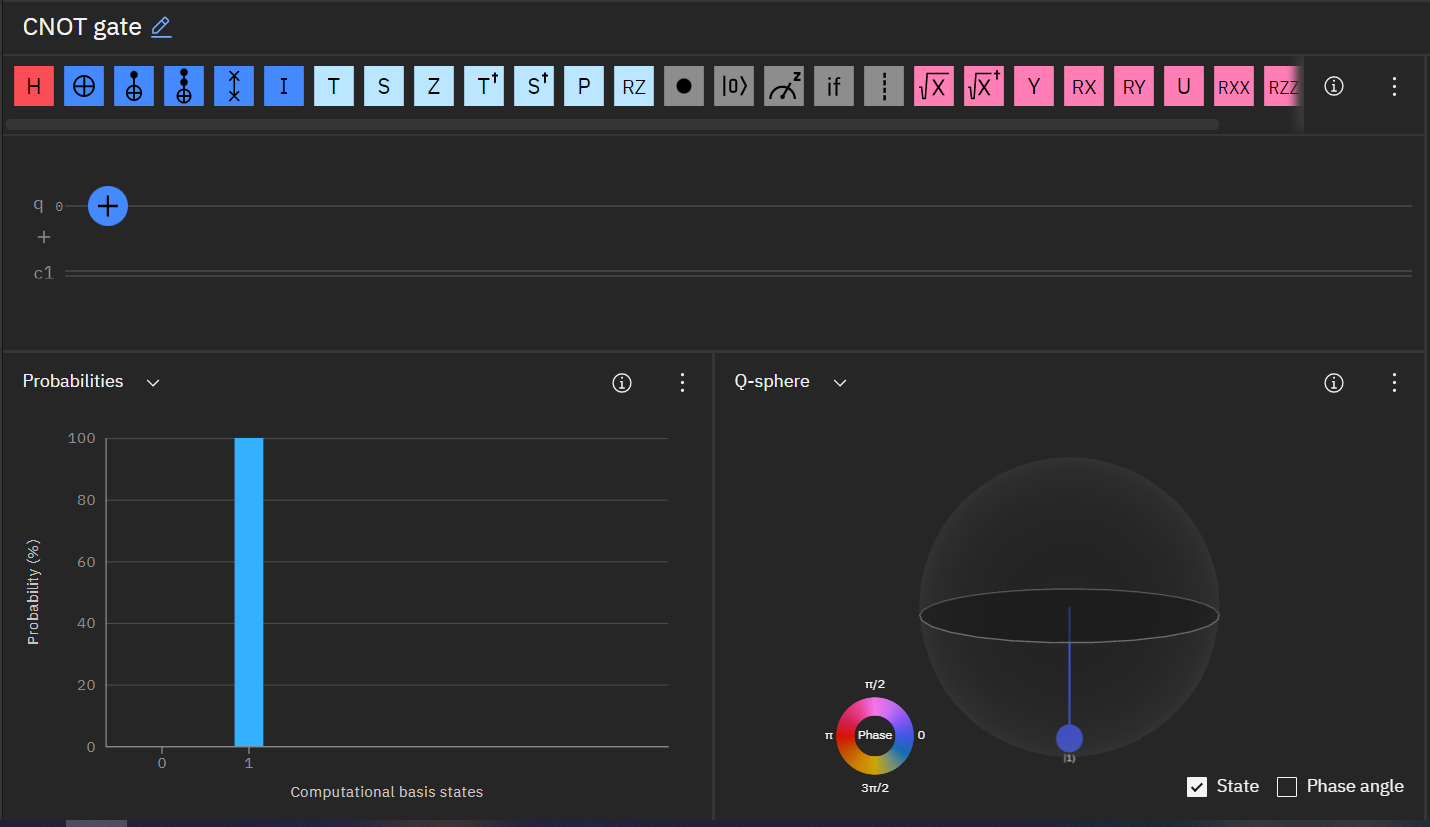
\includegraphics[scale=0.4]{figures/gate-x.png}
	\caption{Circuito con puerta de Hadamard}
\end{figure}

Recordemos que en el Quantum Composer de IBM todos los qubits empiezan siempre en el estado $|0\ra$. Tras aplicarlo a nuestro qubit una puerta $X$ obtendremos $|1\ra$.

\paragraph*{Puerta Hadamard}

Finalmente presentamos la puerta de Hadamard para un único bit. Está descrita por la siguiente matriz unitaria:

\[
	H_1 = \frac{1}{\sqrt 2}
	\begin{pmatrix}
		1 & 1 \\
		1 & -1 
	\end{pmatrix}
\]

Uno de sus usos más comunes es la superposición de qubits. Si aplicamos esta puerta al estado $|0\ra$ obtenemos el estado de Bell:

\[
	H|0\ra = \frac{1}{\sqrt 2} |0\ra + \frac{1}{\sqrt 2} |1\ra = |+\ra
\]

Mientras que si se la aplicamos al estado $|1\ra$ obtenemos:

\[
	H|1\ra = \frac{1}{\sqrt 2} |0\ra - \frac{1}{\sqrt 2} |1\ra = |-\ra
\]

Que también supone una superposición exacta de $|0\ra$ y $|1\ra$ puesto que $|1/\sqrt 2|^2 = |-1/\sqrt 2|^2 = 1/2$.

Podemos estudiar el comportamiento de esta puerta utilizando el Quantum Composer de IBM:

\begin{figure}[H]
	\centering
	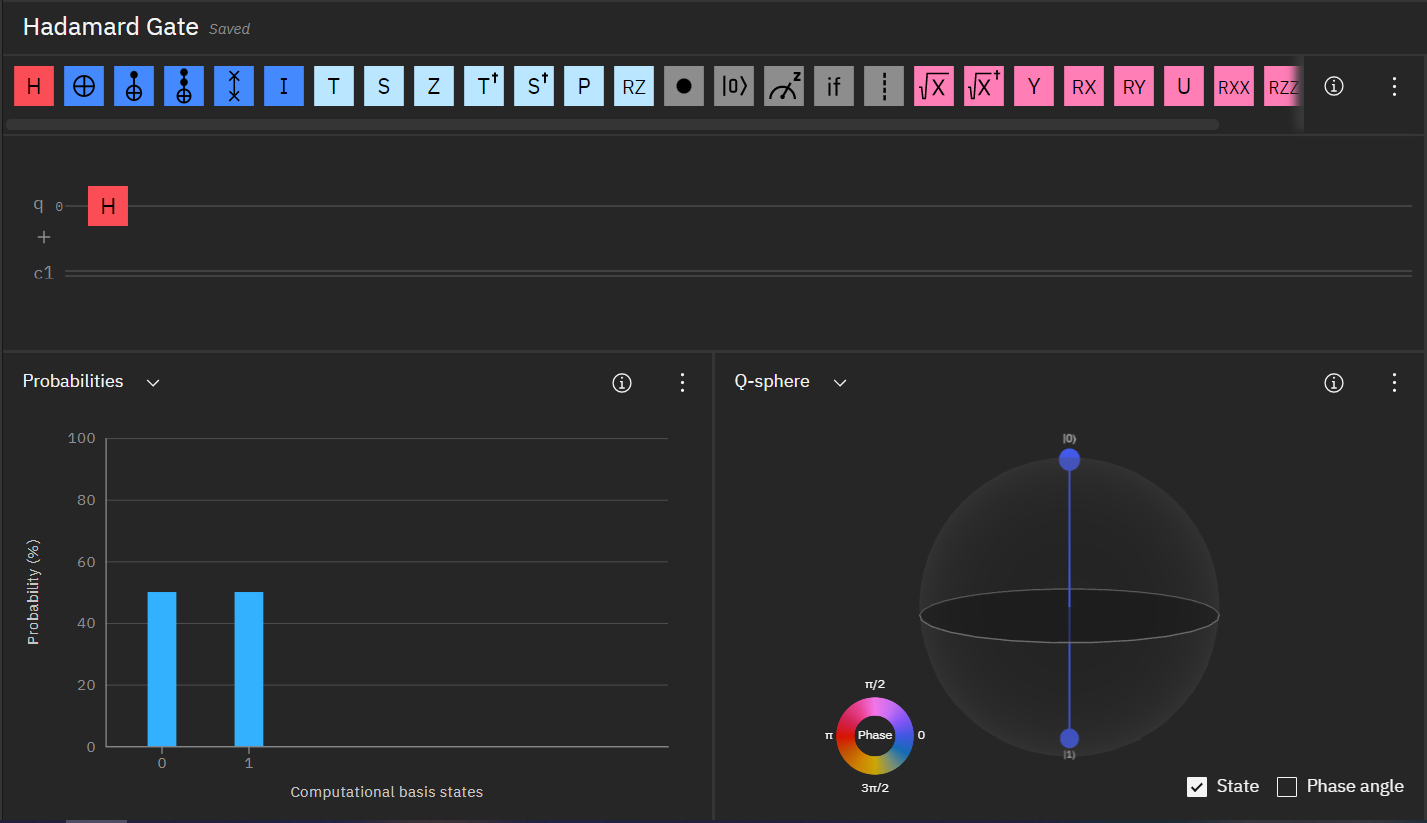
\includegraphics[scale=0.4]{figures/gate-hadamard.png}
	\caption{Circuito con puerta de Hadamard}
\end{figure}

Mirando tanto la \href{URL}{esfera de Bloch} como las probabilidades vemos que tenemos la misma probabilidad de medir $0$ y $1$.

\paragraph*{Puertas de Pauli}

Un conjunto particularmente relevante de puertas son las descritas por las \text{matrices de Pauli}:

\[
X =
	\begin{pmatrix}
		0 & 1 \\
		1 & 0 
	\end{pmatrix}; \quad
	Y =
	\begin{pmatrix}
		0 & -i \\
		i & 0 
	\end{pmatrix}; \quad
	Z =
	\begin{pmatrix}
		1 & 0 \\
		0 & -1 
	\end{pmatrix}
\]

Ya conocemos la matriz $X$, descrita también como la puerta NOT quántica.

\paragraph*{Puertas $T$}

La puerta $\pi/8$, normalmente descrita por la letra $T$, es una \emph{puerta de fase}. Las puertas de fase son un tipo especial de puertas cuánticas que llevan $|0\ra \mapsto |0\ra$ y $|1\ra \mapsto e^{i\phi}|1\ra$, donde $\phi$ es un ángulo de giro. El término $e^{i\phi}$ se denomina \emph{fase} y no afecta a los resultados de las mediciones $0$ y $1$. En particular, la puerta $T$ cumple $\phi = \pi/4$, y la puerta $Z$ de Pauli es una puerta fase con $\phi = \pi/2$:

\[
	T =
	\begin{pmatrix}
		1 & 0 \\
		0 & e^{i\frac{\pi}{4}}
	\end{pmatrix}; \quad
	Z =
	\begin{pmatrix}
		1 & 0 \\
		0 & e^{i\frac{\pi}{2}} = -1
	\end{pmatrix}
\]

En computación clásica, uno de los resultados básicos más relevante es que cualquier función booleana puede describirse utilizando únicamente las puertas clásicas AND, OR y NOT. De la misma forma, en computación cuántica se obtiene siguiente resultado

\begin{theorem}
	Toda matriz unitaria puede aproximarse con una combinación de puertas Hadamard, CNOT y $\pi/8$.
\end{theorem}

Esto es, todo circuito cuántico puede describirse utilizando únicamente dichas puertas.


\subsection{Generación de números aleatorios con un Computador Cuántico}


TODO: añadir enunciado

Sabemos que utilizando la puerta de Hadarmad $H$ explicada en el apartado anterior ponemos un qubit $|0\ra$ en superposición:

\[
	H|0\ra = \frac{1}{\sqrt 2} |0\ra + \frac{1}{\sqrt 2} |1\ra
\]

Si ahora medimos este qubit obtendremos $|0\ra$ con probabilidad $|1/\sqrt 2|^2 = 1/2$, y $|1\ra$ con probabilidad $1/2$. Esto es, hemos creado un generador de bits aleatorios utilizando un único qubit. Para crear un generador de 3 bits utilizaremos un sistema de 3 qubits. Inicialmente en el estado $|000\ra$, aplicaremos una puerta Hadamard a cada qubit de forma independiente, poniendo así cada qubit en superposición:

\[
	\hat H_8|00000000\ra = \frac{1}{\sqrt{2^8}}(|0000000\ra + |00000001\ra + \ldots + |11111111\ra)
\]

Donde la puerta $H_8$ tranformación de Hadamard para ocho qubits. Se puede definir recursivamente de la siguiente forma:

\[
	H_m = H_1 \times H_{m-1}, H_1 = \frac{1}{\sqrt 2}
	\begin{pmatrix}
		1 & 1 \\
		1 & -1 
	\end{pmatrix}
\]

Pasamos a realizar un estudio empírico del circuito diseñado. Lo implementamos utilizando el Quantum Composer de IBM:

\begin{figure}[H]
	\centering
%	\includegraphics[scale=0.8]{figures/3bit_rand_result.png}
\end{figure}

Este simple circuito cuántico pone todos los qubits en superposición y después mide el resultado. Ejecutamos el experimento en el simulador del ordenador cuántico de IBM, obteniendo los siguientes resultados:

\begin{figure}[H]
	\centering
	%\includegraphics[scale=0.8]{figures/3bit_rand.png}
	\caption{Circuito de generación de números aleatorios con 3 bits}
\end{figure}

Estas mediciones han de aproximarse a una uniforme de parámetro $1/256$. Podemos apreciar en la gráfica como los resultados son cercanos a este valor pero distan mucho de definir claramente una uniforme. Podemos comparar estos resultados con la generación de números aleatorios utilizando \emph{scipy} en nuestra propia máquina:

\begin{figure}[H]
	\centering
%	\includegraphics[scale=0.8]{figures/3bit_rand_result.png}
	\caption{Resultados de la simulación con 1024 ejecuciones}
\end{figure}

Comparando ambas gráficas podemos apreciar como la generación de números se acerca a la distribución uniforme mencionada pero en ambas estamos relativamente lejos del modelo teórico. Tras ver los resultados de esta generación utilizando \emph{scipy} podemos asegurar que el generador utilizando el Quantum Composer de IBM obtiene números aleatorios razonablemente aleatorizados.


\subsection{Entrelazamiento}


En este apartado explicaremos en detalle el siguiente circuito cuántico:

\begin{figure}[H]
	\centering
%	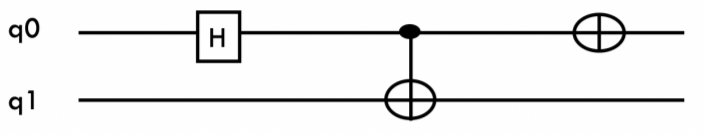
\includegraphics[scale=0.8]{figures/entanglement_statement.png}
\end{figure}

Comenzaremos estudiando un circuito ligeramente más sencillo que también produce entrelazamiento cuántico:

\begin{figure}[H]
	\centering
%	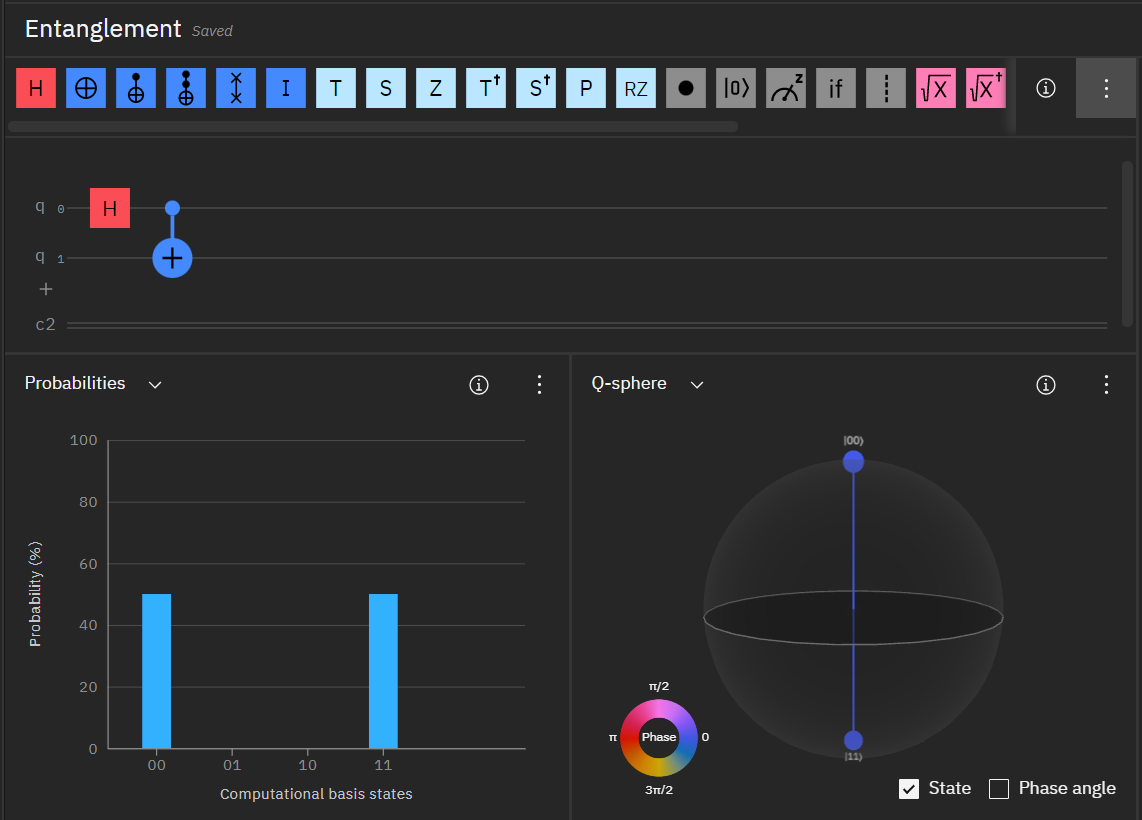
\includegraphics[scale=0.8]{figures/entanglement.png}
\end{figure}

Conociendo ya la puerta de Hadamard, sabemos que el resultado tras la aplicación de dicha puerta al estado $|0\ra$ será $|+\ra$. Utilizando a continuación la puerta CNOT, como el estado de control tiene la misma probabilidad de ser $|0\ra$ que $|1\ra$, el segundo qubit tendrá la misma probabilidad de tener dichos valores. Analíticamente:

\[
	|+\ra|0\ra CNOT = \frac{|00\ra + |11\ra}{\sqrt 2} = |\Phi^+\ra
\]


Obteniéndo así el famoso estado EPR (Einstein, Podolsky y Rosen) o estado de Bell $|\Phi^+\ra$. En este aparentemente sencillo estado puede apreciarse el entrelezamiento cuántico, lo que dió lugar a dicha paradoja. Estudiémos este estado en detalle.

Para empezar, al medir ambos qubits únicamente podremos obtener los resultados $00$ y $11$. Si únicamente medimos uno de los dos qubits y obtenemos, por ejemplo, un $0$, entonces cuando midamos el otro estado obtendremos otro $0$ con toda probabilidad, pues los únicos resultados finales válidos son los anteriormente descritos $00$ y $11$. Lo mismo ocurre si medimos $1$: el valor del segundo qubit ha de ser también un $1$.

De esta forma, hemos hecho que el segundo qubit colapse a un estado al medir otro qubit distinto. Estas son las implicaciones del entrelazamiento cuántico.

Estudiémos ahora el circuito del enunciado:

\begin{figure}[H]
	\centering
%	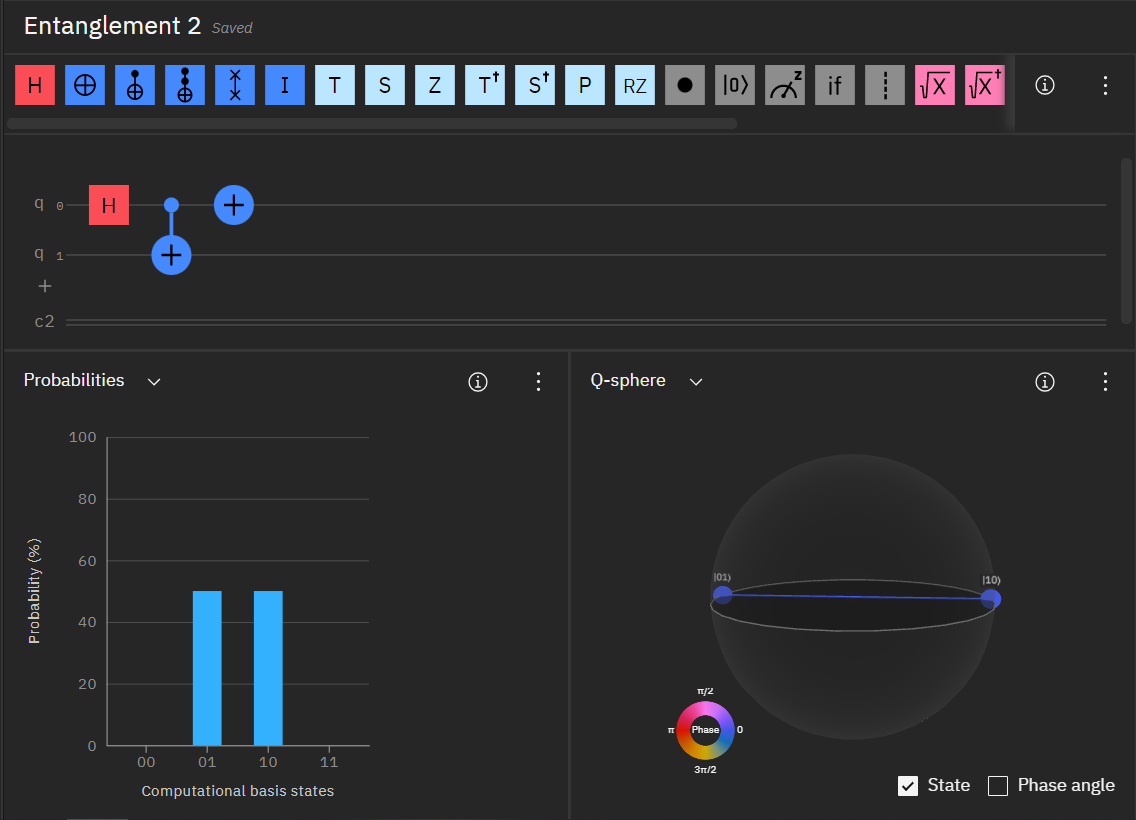
\includegraphics[scale=0.8]{figures/entanglement2.png}
\end{figure}

Esto es, aplicarle una puerta NOT al primer qubit del estado de Bell, obteniendo:

\[
	\frac{|00\ra + |11\ra}{\sqrt 2} (NOT \times \I) = \frac{|10\ra + |01\ra}{\sqrt 2}
\]

Este estado se comporta como el anterior pero con valores de medida opuestos: si medimos un $0$ en el primer qubit, el segundo colapsará automáticamente al estado $1$, y viceversa.

\subsection{Sumador de 2 qbits}

TODO: enunciado

\begin{figure}[H]
	\centering
	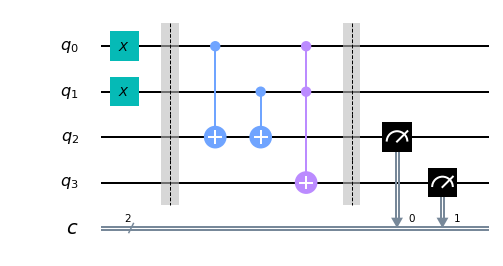
\includegraphics[scale=0.8]{figures/sumator_statement.png}
\end{figure}


\section{Ejercicios opcionales de la práctica 2}

\end{document}
